\section{Úvod}
Tento dokument slouží k dokumentaci projektu IMP na téma Meteostanice.
Meteostanice byla realizována na desce Wemos D1 R32 s OLED displejem SSD1306
a senzorem teploty a vlhkosti SHT-31 pomocí vývojového prostředí PlatformIO.

Pro realizaci byly využity již existující knihovny pro displej
\cite{ssd1306} i senzor \cite{sht3x}, které obsahují funkce pro
inicializaci I2C a komunikaci s jednotlivými komponenty.
Knihovna pro displej byla upravena (odebrány některé funkce; konkrétně pro
inicializaci a komunikaci přes rozhraní SPI) pro potřeby projektu.
Mj. byly využity \textit{RTOS} funkce pro vytvoření \textit{tasků}.

Bylo použito následující zapojení:
\begin{itemize}
	\item D16 - SDA (displej a senzor)
	\item D17 - SCL (displej a senzor)
	\item 3V3 - VCC (displej a senzor)
	\item GND (1) - GND (displej)
	\item GND (2) - GND (senzor)
\end{itemize}

\begin{figure}[h!]
	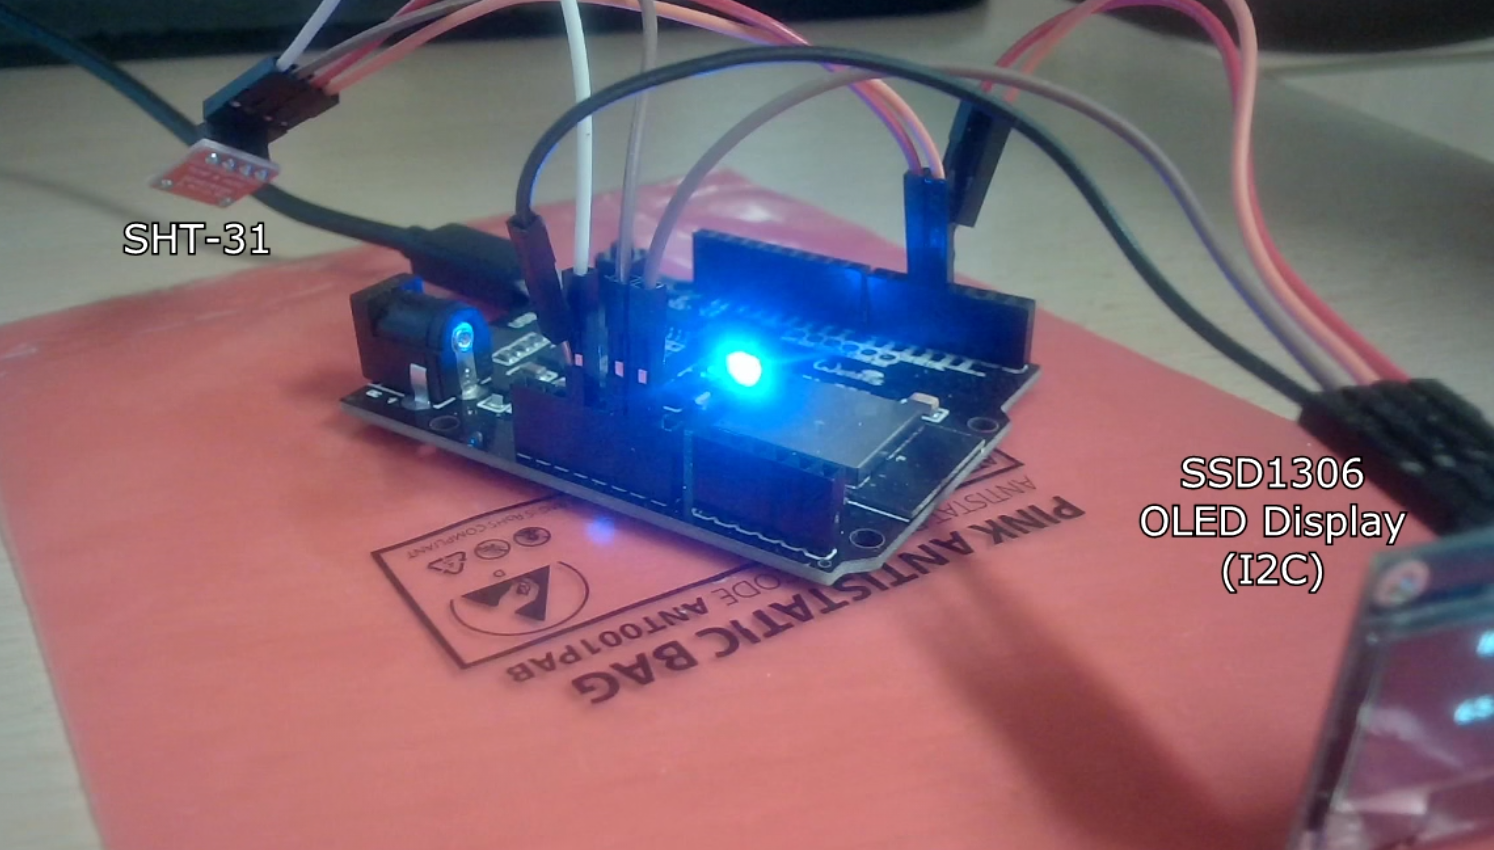
\includegraphics[width=1.0\textwidth]{connection.png}
	\caption{Zapojení senzoru a displeje (breadboard nebyl
	dostupný, proto bylo nutné improvizovat)}
\end{figure}
